%% Welcome to OverLyX — the personal example document (packages/server/templates/welcome).
\documentclass[english]{article}
\usepackage[T1]{fontenc}
\usepackage[utf8]{inputenc}
\usepackage{color}
\usepackage{babel}
\usepackage{amsmath}
\usepackage{amssymb}
\usepackage{graphicx}
\usepackage[authoryear]{natbib}
\usepackage[pdfusetitle,
 bookmarks=true,bookmarksnumbered=false,bookmarksopen=false,
 breaklinks=false,pdfborder={0 0 0},pdfborderstyle={},backref=false,colorlinks=true]
 {hyperref}
\hypersetup{
 linkcolor=blue,citecolor=blue,urlcolor=blue}

\makeatletter
%%%%%%%%%%%%%%%%%%%%%%%%%%%%%% User specified LaTeX commands.
@@LLANGLE@@

\makeatother

%% OverLyX ------------------------------------------------------------------
%% overlyx-settings: {"textclass":"article","cite_engine":"natbib","cite_engine_type":"authoryear","biblio_style":"plainnat","output_changes":"false","use_hyperref":"true","justification":"default","use_package":{"cancel":"0","esint":"0","mathdots":"0","mathtools":"0","mhchem":"0","stackrel":"0","stmaryrd":"0","undertilde":"0"}}
%% Packages and macros needed by the content (generated on every save; put your own preamble above this block).
\makeatletter
\providecommand{\LyX}{\texorpdfstring{\ensureascii{%
  L\kern-.1667em\lower.25em\hbox{Y}\kern-.125emX\@}}{LyX}}
\DeclareRobustCommand*{\lyxarrow}{%
\@ifstar
{\leavevmode\,$\triangleleft$\,\allowbreak}
{\leavevmode\,$\triangleright$\,\allowbreak}}
%% Because html converters don't know tabularnewline
\providecommand{\tabularnewline}{\\}
\makeatother
%% end OverLyX --------------------------------------------------------------

\begin{document}
\title{Welcome to OverLyX}
\author{@@NAME@@}
\maketitle
\begin{abstract}
This is your personal example document, @@FIRSTNAME@@. It is an ordinary \LyX{} file in a project of your own: everything you do here is saved exactly as \LyX{} would save it, so you can open it in desktop \LyX{} at any time. Edit it, break it, share it --- or delete the project once you know your way around.
\end{abstract}

\section{Editing text}\label{sec:text}

Every paragraph has a \emph{layout} --- Standard, Section, Itemize, Quote, \ldots{} --- chosen from the drop-down at the left of the toolbar, with \LyX 's shortcuts (\textsf{Alt+P} followed by a letter, e.g.\textsf{ Alt+P 2} for a section), or from the right-click menu. The outline on the right follows the sections; click an entry to jump there.

Character styles work as in \LyX : \emph{emphasis} with\textsf{ Ctrl+E}, \textbf{bold} with\textsf{ Ctrl+B}, \texttt{typewriter} and small caps from the Edit\lyxarrow Text Style menu. Footnotes\footnote{A footnote. Insets like this one open and close with a click on their label; \textsf{Ctrl+Alt+F} inserts one.} and ``typographic quotes'' are insets, just like in \LyX .
\begin{itemize}
\item Lists are layouts too: this is an Itemize paragraph (\textsf{Alt+P I}).
\item Press\textsf{ Enter} for the next item, \textsf{Tab} to nest it one level deeper, and\textsf{ Shift+Tab} (or the layout drop-down) to get out again.
\end{itemize}
\begin{enumerate}
\item Enumerate (\textsf{Alt+P E}) numbers its items ---
\item and Description (\textsf{Alt+P D}) sets the first words in bold, like the shortcut list below.
\end{enumerate}
\begin{description}
\item [{Ctrl+M}] inline formula
\item [{Ctrl+Shift+M}] display formula
\item [{Ctrl+R}] compile the PDF
\item [{Ctrl+F}] find and replace
\item [{Ctrl+Shift+E}] track changes
\end{description}
Cross-references are insets as well: the mathematics are in Section \ref{sec:math}, the figure is Figure \ref{fig:waves} and the shortcuts are collected in Table \ref{tab:shortcuts}. Insert\lyxarrow Label puts a label on the current paragraph; Insert\lyxarrow Cross-reference lists all labels of the project, including those of child documents.

\section{Mathematics}\label{sec:math}

Formulas are edited in place with a port of \LyX 's math editor, so everything behaves as you are used to: \textsf{Ctrl+M} starts an inline formula such as $e^{i\pi}+1=0$ and\textsf{ Ctrl+Shift+M} a displayed one. Type a backslash to enter a command (\texttt{\textbackslash int}, \texttt{\textbackslash alpha}, \texttt{\textbackslash frac}), complete it with\textsf{ Tab}, and use\textsf{ Space} to leave the current inset:

\begin{equation}
\int_{-\infty}^{\infty}e^{-x^{2}}\,\mathrm{d}x=\sqrt{\pi}.\label{eq:gauss}
\end{equation}

The math toolbars (they appear while the cursor is in a formula) hold the Greek letters, operators, relations, arrows, decorations, fonts and delimiters of \LyX 's panels. Delimiters come in every size --- plain, \texttt{\textbackslash left}\ldots\texttt{\textbackslash right}, \texttt{\textbackslash big}, \texttt{\textbackslash Big}, \texttt{\textbackslash bigg}, \texttt{\textbackslash Bigg} --- including the double angle brackets, for which OverLyX added a small macro to this document's preamble:

\begin{equation}
\left\llangle f,g\right\rrangle =\int_{0}^{1}f(x)\,g(x)\,\mathrm{d}x,\qquad\bigl\llangle x\bigr\rrangle \neq\left|x\right|.\label{eq:llangle}
\end{equation}

Document macros are honoured. The following paragraph defines one --- a \LyX{} math macro (Insert\lyxarrow Math\lyxarrow Macro) with one argument:

\global\long\def\E#1{\mathbb{E}\left[#1\right]}%

From here on $\E{X}$ expands to the definition (editable in place, argument included); equation (\ref{eq:macro}) uses it, and the definition travels with the document to \LaTeX .

\begin{align}
\mathrm{Var}\left[X\right] & =\E{X^{2}}-\E{X}^{2},\label{eq:macro}\\
\mathrm{Cov}\left[X,Y\right] & =\E{XY}-\E{X}\E{Y}.\nonumber 
\end{align}

Press\textsf{ Enter} inside a formula to add a row (an inline formula becomes an\texttt{ align} environment), \textsf{Tab} to move between cells, and use the matrix button of the math toolbar for something like $\begin{pmatrix}a & b\\ c & d \end{pmatrix}$. The right-hand \emph{ Source} panel shows the \LyX{} and \LaTeX{} source of the paragraph under the cursor.

\section{Figures, tables and references}\label{sec:floats}

Figure \ref{fig:waves} is a floating figure with a PDF graphic from the project's\texttt{ figures} folder. Upload your own files with the upload button next to a project in the file browser (or drop them onto it); SVG, PNG, JPEG, PDF and EPS are rendered in the editor and converted for \LaTeX{} as needed.

\begin{figure}
\begin{centering}
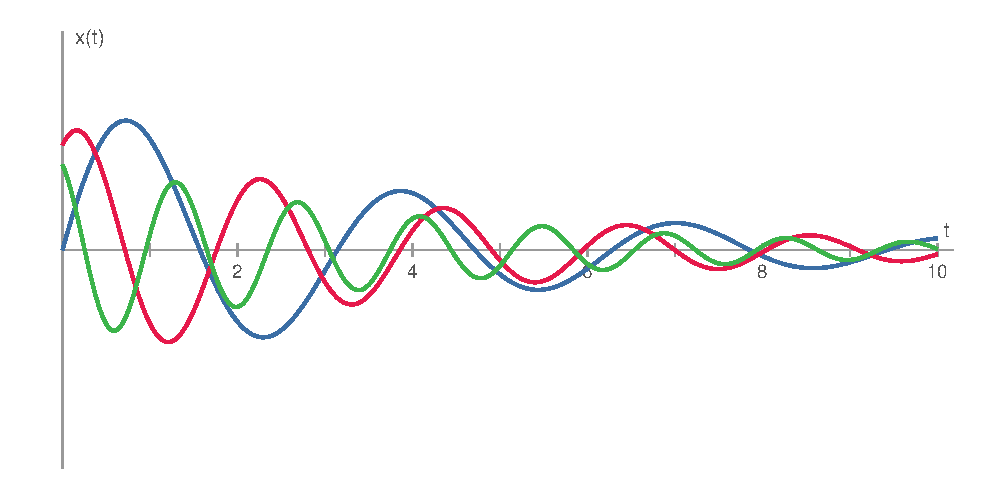
\includegraphics[width=0.7\columnwidth]{figures/waves.pdf}
\par\end{centering}
\caption{Three damped oscillations, $x(t)=A\,e^{-t/4}\sin(\omega t+\varphi)$. The figure is\texttt{ figures/waves.pdf} in this project; double-click it to change its size.}\label{fig:waves}
\end{figure}

Tables are \LyX{} tables: the table toolbar (shown while the cursor is in a table) adds and removes rows and columns, sets borders and alignment, and joins cells.

\begin{table}
\caption{Keyboard shortcuts you will use most (Help\lyxarrow Keyboard shortcuts lists them all).}\label{tab:shortcuts}

\centering{}%
\begin{tabular}{ll}
\hline 
Keys & Action\tabularnewline
\hline 
\textsf{Ctrl+M} / \textsf{Ctrl+Shift+M} & inline / display formula\tabularnewline
\textsf{Alt+P} + letter & paragraph layout (1--6 sections, I, E, D lists)\tabularnewline
\textsf{Ctrl+E}, \textsf{Ctrl+B} & emphasis, bold\tabularnewline
\textsf{Ctrl+R} & compile the PDF\tabularnewline
\textsf{Ctrl+Shift+E} & track changes on/off\tabularnewline
\textsf{Ctrl+Alt+F} / \textsf{Ctrl+Alt+N} / \textsf{Ctrl+Alt+C} & footnote / note / comment\tabularnewline
\textsf{Ctrl+F} & find and replace\tabularnewline
\hline 
\end{tabular}
\end{table}

Citations come from the project's BibTeX files (\texttt{refs.bib} here): Insert\lyxarrow Citation searches them by author, year and title. OverLyX writes \LyX{} files, \LyX{} writes \LaTeX{} \citep{lamport1994}, and underneath it all is \TeX{} \citep{knuth1984}. Concurrent edits from several people are merged with conflict-free replicated data types \citep{shapiro2011}, which is why nobody ever has to resolve a merge conflict.

\section{Working together}\label{sec:collab}

\textbf{Sharing.} A project is private to you until you share it --- like a Google Doc. File\lyxarrow Share project\ldots{} (or the share button next to the project in the file browser) invites people by username or e-mail address as\emph{ viewers} or \emph{ editors}, and can turn on a link that anyone signed in can use. Someone invited by e-mail gets access the moment they sign in with Google.

\textbf{Presence.} Everybody who has the document open appears as a small avatar in the status bar, and their cursors and selections show in the text in their colour. Click an avatar to jump to where that person is editing.

\textbf{Saving.} There is no Save button: every change goes to the server as you type and is written to the\texttt{ .lyx} file a moment later (the status bar says \emph{ All changes saved}). If you open the same file in desktop \LyX{} and save it there, OverLyX picks up the change. Working offline is fine too --- edits are kept in the browser and merge when you are back.

\textbf{Changes, notes and comments.} \textsf{Ctrl+Shift+E} turns on change tracking; the review toolbar walks through the changes and accepts or rejects them, just as in \LyX . Notes are invisible in the output --- this one is a \LyX{} note: %
%% @note
%% A \LyX{} note. It is stored in the file and shown in desktop \LyX , but never printed.
%% @end
Comments become discussion threads (reply, resolve), and View\lyxarrow Notes \& comments in the margin shows them next to the text: %
%% @comment
%% OverLyX (2026-08-28 09:00):
%%
%% A comment thread. Click it to reply or to mark it resolved.
%% @end
File\lyxarrow Versions keeps named versions and automatic snapshots of the document; any of them can be compared and restored.

\section{Compiling and exporting}\label{sec:compile}

\textsf{Ctrl+R} compiles the document with\texttt{ pdflatex} (via\texttt{ latexmk}) in the background and shows the result in the PDF panel; errors and warnings are listed underneath it. File\lyxarrow Export also offers the \LaTeX{} source, a build with native \LyX{} for comparison, and the\texttt{ .lyx} file itself for download. Document\lyxarrow Settings changes the class, the preamble, packages and the bibliography style.

\section{Where to go next}\label{sec:next}

Create a project of your own with the\textbf{ + Project} button in the file browser and upload your existing\texttt{ .lyx} files, figures and bibliographies --- or ask a colleague to share theirs with you. Help\lyxarrow Keyboard shortcuts lists everything; the source of this editor is at\href{https://github.com/japhba/overlyx}{github.com/japhba/overlyx}.

Enjoy writing, @@FIRSTNAME@@!

\bibliographystyle{plainnat}
\bibliography{refs}

\end{document}
